\section{Dataset}

Here we'll present our dataset just like in the survey paper and we'll present a bunch of statistics about it.

\subsection{Raw Format}
We talk about how the dataset was constructed, that it was constructured by non data scientists, that it was in exceel files and in a format not appropriate for training.

Annotations are shifted, videos don't start immediately on the climbing but often begin with some sort of synchronization sequence.

\subsection{Chosen Structure}
Here we state the different possible structures \& present the choosen one.

\subsection{Developed Tools \& Easier Training}

\href{https://github.com/raideno/cached-dataset}{https://github.com/raideno/cached-dataset}
\href{https://github.com/raideno/video-dataset}{https://github.com/raideno/video-dataset}

\subsection{Statistics, Illustrations \& Data Exploration}

\begin{figure}[ht]
    \centering
    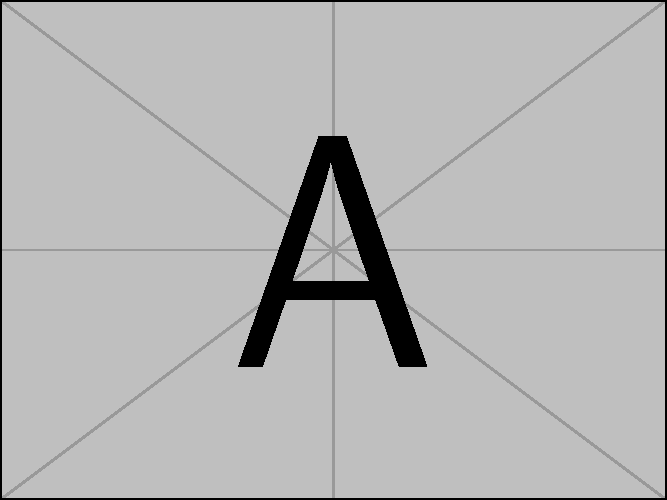
\includegraphics[width=8.4cm]{assets/mwe/example-image-a}
    \caption{Your caption here.}
    \label{fig:example}
\end{figure}

Showcase some example image, sequence of frames \& videos of the dataset.

Display some plots that showcase the dataset statistics and analyze and talk about these statistics.

\subsection{Optimization}

\todo[inline]{This section was intended for talking about the cached-dataset and how we used it to avoid re-extracting the features each time, but we'll probabily discard it and move it lower as we haven't introduced the model yet to talk about caching and optimizing it's training.}

\subsection{Other Datasets}

Talk about other popular datasets in the field, their sizes and magnitude, where they are speciliazed, by who and why they have been created and the kind of videos we can find in them.